%********************************************
% Lab 02: Converting Boolean Logic to a Circuit
%********************************************
\chapter{Boolean Logic}

\section{Purpose}

This lab has three goals: 

\begin{itemize}
	\item Design circuits when given a Boolean expression.
	\item Create subcircuits.
	\item Create and exercise a test of the subcircuits.
\end{itemize}

\LE permits designers to work with a main circuit and any number of subcircuits. Students who have studied programming languages are familiar with ``functions'' or ``classes'' that can be designed and built one time and then reused many times whenever they are needed. \LE permits that same type of modular design by using subcircuits. 

The \LE starter for this lab includes a \lstinline[columns=fixed]|main| circuit and one subcircuit, named \lstinline[columns=fixed]|Equation_1|. The starter subcircuit is used to practice creating a circuit from a Boolean expression and then a new subcircuit is added and a second Boolean expression is used to build that circuit.

\section{Procedure}

\subsection{Subcircuit: Equation 1}

\marginpar{A magnifying glass icon is used to indicate which circuit is active on the drawing canvas.}The starter circuit includes a subcircuit named \lstinline[columns=fixed]|Equation_1|. Double-click that circuit in the Explorer Pane to activate it. The drawing canvas for this subcircuit is mostly blank except for a Boolean expression: $ (A'BC')+(AB'C')+(ABC) $. Before starting to design a circuit, it is helpful to take a minute to analyze the expression. 

\begin{itemize}
	\item There are only three variables used in the entire expression: \textit{A}, \textit{B}, and \textit{C}. Therefore, there would be three inputs into the circuit.
	\item There are three groups of variables and within each group the variables are joined with an \texttt{AND}. Therefore, the circuit must include three \texttt{AND} gates with three inputs for each gate.
	\item The three groups of variables are joined with an \texttt{OR}. Therefore, the circuit must include an \texttt{OR} gate with three inputs.
	\item While the expression does not name an output variable, it is reasonable to assume that the circuit would output a logic 1 or 0. Therefore, a one-bit output variable must be specified.
\end{itemize}

\marginpar{Do not be concerned with the exact placement of components on the drawing canvas. They can be rearranged as the build progresses.}Start by placing three inputs and an output on the drawing canvas. Inputs are indicated by a green icon with \textit{I->} on the tool bar above the drawing canvas. Click that tool and place three input pins named \textit{In1A}, \textit{In1B}, and \textit{In1C} \textemdash that means ``Input for Equation One, variable A'' and so forth. 

Outputs are indicated by a white icon with \textit{->O} found on the tool bar above the drawing canvas. Click that tool and place an output named \textit{Out1}. The circuit should look like Figure \ref{fig:02-01}.

\begin{figure}[H]
	\centering
	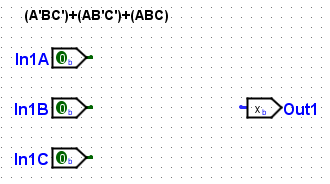
\includegraphics[width=\maxwidth{.95\linewidth}]{gfx/02-01}
	\caption{Equation 1 Inputs-Outputs}
	\label{fig:02-01}
\end{figure}

\marginpar{The gates in this manual are all ``narrow'' size. The size does not change the gate behavior but makes it easier to wire the complex circuits in later labs.}Next, the gates should be added. The \texttt{AND} gate tool can be found on the tool bar. Click that tool and place three \texttt{AND} gates on the circuit. Click each gate and in its properties panel set the \textit{Number of Inputs} to 3. 

The \texttt{OR} gate tool can be found on the tool bar. Click that tool and place one \texttt{OR} gate on the circuit. Click that gate and in its properties panel set the \textit{Number of Inputs} to 3.

The circuit should look like Figure \ref{fig:02-02}.

\begin{figure}[H]
	\centering
	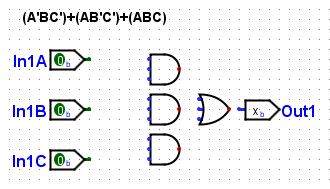
\includegraphics[width=\maxwidth{.95\linewidth}]{gfx/02-02}
	\caption{Equation 1 And-Or Gates}
	\label{fig:02-02}
\end{figure}

Next, the inputs for the \texttt{AND} gates should be set to match the Boolean expression. The top \texttt{AND} gate will match the first group of inputs, $ (A'BC') $, so inputs \textit{A} and \textit{C} should be negated. To negate those two inputs, click the \texttt{AND} gate and in the properties panel set the \textit{Negate} item for the top and bottom input to ``Yes.'' When that is done, the two inputs on the \texttt{AND} gate should include a small ``negate'' circle.

In the same way, the middle and bottom input for the second \texttt{AND} gate should also be negated. The circuit should look like Figure \ref{fig:02-03}.

\begin{figure}[H]
	\centering
	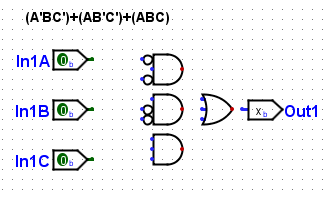
\includegraphics[width=\maxwidth{.95\linewidth}]{gfx/02-03}
	\caption{Equation 1 And Gate Inputs Set}
	\label{fig:02-03}
\end{figure}

Finally, connect all gates with wires, like Figure \ref{fig:02-04}. 

\begin{figure}[H]
	\centering
	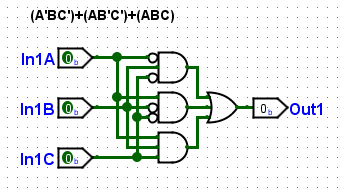
\includegraphics[width=\maxwidth{.95\linewidth}]{gfx/02-04}
	\caption{Equation 1 Circuit Completed}
	\label{fig:02-04}
\end{figure}

Test the circuit by selecting the \textit{poke} tool in the tool bar (it looks like a pointing finger) and setting various combinations of 1 and 0 on the three inputs. The output pin should go high only when the inputs are set to $ (A'BC') $, $ (AB'C') $, or $ (ABC) $.

\subsection{Subcircuit: Equation 2}

A new subcircuit can be added to a circuit by clicking \textsc{Project -> Add Circuit}. Name the new circuit \lstinline[columns=fixed]|Equation_2|. Open the new subcircuit by double-clicking its name in the Explorer Pane. 

Because this is a new subcircuit, the drawing canvas is blank. To start this subcircuit, write the equation for the circuit near the top of the drawing canvas by clicking the ``A'' button on the Toolbar and then clicking near the top of the drawing canvas and typing the following:

\[ (A'B'CD')+(A'BCD)+(AB'CD')+(ABCD') \]

It will save time to take a few minutes and analyze the expression. 

\begin{itemize}
	\item There are only four variables used in the entire expression: \textit{A}, \textit{B}, \textit{C}, and \textit{D}. Therefore, there would be four inputs into the circuit.
	\item There are four groups of variables and within each group the variables are joined with an \texttt{AND}. Therefore, the circuit must include four \texttt{AND} gates with four inputs for each gate.
	\item The four groups of variables are joined with an \texttt{OR}. Therefore, the circuit must include an \texttt{OR} gate with four inputs.
	\item While the expression does not name an output variable, it is reasonable to assume that the circuit would output a logic 1 or 0. Therefore, a one-bit output variable must be specified.
\end{itemize}

Design the subcircuit using these names for the inputs: \textit{In2A}, \textit{In2B}, \textit{In2C}, and \textit{In2D}. Also include an output named \textit{Out2}. Set the \texttt{AND} gates so the their inputs are negated properly and then wire the entire subcircuit. Finally, test the circuit to ensure the output goes high only when the four specified combinations of inputs are present.

\subsection{Main Circuit}

Make the \lstinline[columns=fixed]|main| circuit active by double-clicking its name in the Explorer Panel. Click once on the \lstinline[columns=fixed]|Equation_1| circuit and the cursor will change into an image of that circuit as it will appear on the drawing canvas. Click on the drawing canvas to drop that subcircuit. The circuit can later be moved by clicking it and dragging it to a new location. Wire the three inputs and output as shown in Figure \ref{fig:02-05}. Notice that the input/output pins do not need to be named the same as in the subcircuit; for example, the output for \lstinline[columns=fixed]|Equation_1| is labeled \textit{Out1} but it is connected to an output pin labeled \textit{True1}.

\begin{figure}[H]
	\centering
	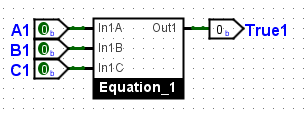
\includegraphics[width=\maxwidth{.95\linewidth}]{gfx/02-05}
	\caption{Main Circuit}
	\label{fig:02-05}
\end{figure}

Add the \lstinline[columns=fixed]|Equation_2| circuit in the same way and wire four inputs and one output to that circuit. The inputs should be labeled \textit{A2}, \textit{B2}, \textit{C2}, and \textit{D2} and the output labeled \textit{True2}.

\subsection{Testing the Circuit}

One way to test this circuit is to use the \textit{poke} tool and click various input combinations for both subcircuits. If the subcircuits are correct then the output will only go high when the correct combination is set on the inputs. However, as digital logic circuits become more complex it is important to automate the testing process so no input combinations are overlooked. \LE includes a \textsc{Simulate -> Test Vector} feature that is used for automating circuit testing.

The first step in using automatic testing is to create a \textit{Test Vector} file. This is a simple \textit{.txt} file that can be created in any text processor, like \textit{Notepad}. \marginpar{Do not use a word processor to create the Test Vector since that would add unneeded codes for things like fonts and margins.} The format for a test vector is fairly simple.

\begin{itemize}
	\item Every line is a single test of the circuit, except the first line.
	\item The first line defines the various inputs and outputs being tested.
	\item Any line that starts with a hash mark (\#) is a comment and is ignored.
\end{itemize}

Following is the test vector file used to test the \lstinline[columns=fixed]|Equation_1| subcircuit.

\begin{Verbatim}[frame=lines,
								 numbers=left,
								 xleftmargin=10mm,
								 xrightmargin=10mm]
# Test vector for Lab 2
# Equation 1
A1 B1 C1 True1
0   0  0     0
0   0  1     0
0   1  0     1
0   1  1     0
1   0  0     1
1   0  1     0
1   1  0     0
1   1  1     1
\end{Verbatim}

Following is an explanation for the \textit{Test vector for Lab 2} file.

\begin{description}
	\item[Line 1] This is just the title of the file. Because this line starts with a hash (\#) it is a comment and will be ignored by \LE.
	\item[Line 2] This is another descriptor line and is ignored by \LE.
	\item[Line 3] This line lists all of the inputs and outputs in the circuit under test. In this case, there are three inputs, \textit{A1}, \textit{B1}, and \textit{C1}, along with one output, \textit{True1}. \LE is able to determine whether the pin is an input or output from its properties. NOTE: each of the inputs and outputs in this circuit are single bits. If an input or output has more than one bit then that must be specified on this line. For example, if \textit{True1} was actually a four-bit output then that pin would be listed as \textit{True1[4]}.
	\item[Line 4] This line contains the first test for the circuit. This line specifies that \LE make \textit{A1}, \textit{B1}, and \textit{C1} equal to zero and then check to be certain that \textit{True1} is also zero.
	\item[Other Lines] All other lines set the three input bits and specify the expected response in the output bit.
\end{description}

The test vector for Equation 2 would look like this:

\begin{Verbatim}[frame=lines,
								 numbers=left,
								 xleftmargin=10mm,
								 xrightmargin=10mm]
# Test vector for Lab 2
# Equation 2
A2 B2 C2 D2 True2
0   0  0  0     0
0   0  0  1     0
0   0  1  0     1
0   0  1  1     0
0   1  0  0     0
0   1  0  1     0
0   1  1  0     0
0   1  1  1     1
1   0  0  0     0
1   0  0  1     0
1   0  1  0     1
1   0  1  1     0
1   1  0  0     0
1   1  0  1     0
1   1  1  0     1
1   1  1  1     0
\end{Verbatim}

In practice, a circuit designer would usually not create two different test vectors but would, instead, create just one file to test all parts of the circuit. Combining the \textit{Equation 1} test and the \textit{Equation 2} test is not quite as easy as appending one after the other since all input and output pins for both circuits must be specified at the top of the file. Following is the test vector for a circuit that combines \textit{Equation 1} and \textit{Equation 2}. Notice that all input and output pins are defined on line three then each line beginning with line four tests both of the equation circuits. Because only eight tests are needed to fully exercise \textit{Equation 1} but 16 are needed for Equation 2, the \textit{Equation 1} tests are repeated starting on Line 12.

\begin{Verbatim}[frame=lines,
								 numbers=left,
								 xleftmargin=10mm,
								 xrightmargin=10mm]
# Test vector for Lab 2
# Equation 1   - Equation 2
A1 B1 C1 True1   A2 B2 C2 D2 True2
0   0  0     0    0  0  0  0     0
0   0  1     0    0  0  0  1     0
0   1  0     1    0  0  1  0     1
0   1  1     0    0  0  1  1     0
1   0  0     1    0  1  0  0     0
1   0  1     0    0  1  0  1     0
1   1  0     0    0  1  1  0     0
1   1  1     1    0  1  1  1     1
0   0  0     0    1  0  0  0     0
0   0  1     0    1  0  0  1     0
0   1  0     1    1  0  1  0     1
0   1  1     0    1  0  1  1     0
1   0  0     1    1  1  0  0     0
1   0  1     0    1  1  0  1     0
1   1  0     0    1  1  1  0     1
1   1  1     1    1  1  1  1     0
\end{Verbatim}

To start a test, click \textsc{Simulate -> Test Vector}. The window illustrated in Figure \ref{fig:02-06} opens. 

\begin{figure}[H]
	\centering
	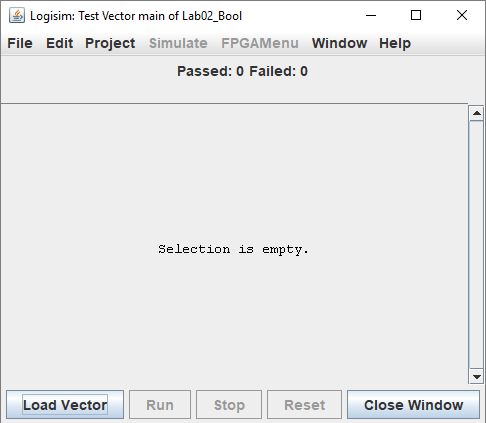
\includegraphics[width=\maxwidth{.95\linewidth}]{gfx/02-06}
	\caption{Test Vector Window}
	\label{fig:02-06}
\end{figure}

Click the \textit{Load Vector} button at the bottom of the window and load the test vector file. The test will automatically start and Logisim-evolution will report the results, like in Figure \ref{fig:02-07}.

\begin{figure}[H]
	\centering
	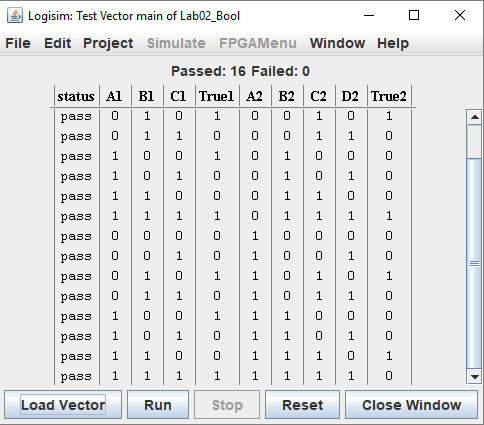
\includegraphics[width=\maxwidth{.95\linewidth}]{gfx/02-07}
	\caption{Test Completed}
	\label{fig:02-07}
\end{figure}

The test indicates all 16 lines passed and zero failed so it could be reasonably concluded that the circuits are functioning properly. Figure \ref{fig:02-08} illustrates a failed test. The circuit designer would then need to troubleshoot to determine what went wrong with the circuit.

\begin{figure}[H]
	\centering
	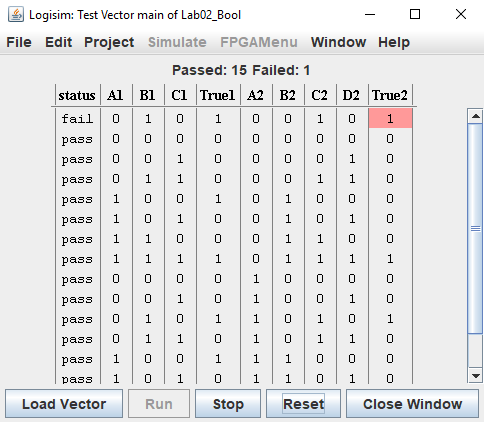
\includegraphics[width=\maxwidth{.95\linewidth}]{gfx/02-08}
	\caption{Test Failure}
	\label{fig:02-08}
\end{figure}

\section{Deliverable}

\marginpar{It is important to name all inputs and outputs as specified in the lab since they are checked with a Test Vector file that depends on those names.}To receive a grade for this lab, complete the \lstinline[columns=fixed]|main| circuit and both subcircuits. Be sure the standard identifying information is at the top left of the \lstinline[columns=fixed]|main| circuit, similar to: 

\bigskip
% The minipage environment keeps the three lines together - no page break.
\begin{minipage}{\linewidth}
	\begin{verbatim}
	George Self
	Lab 02: Boolean Equations
	February 18, 2018
	\end{verbatim}
\end{minipage}
\bigskip

Save the file with this name: \emph{\texttt{Lab02\_Bool}} and submit that file for grading.

